\definecolor{mygray}{RGB}{178, 178, 178}

\begin{solution}{5}
    \begin{figure}
        \centering
        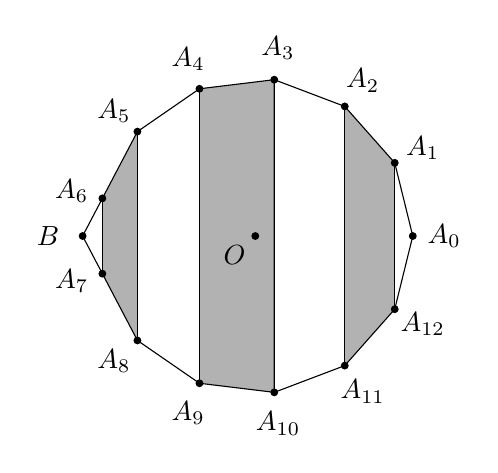
\begin{tikzpicture}
            \foreach \i in {0,...,12} {
                \node (a\i) at ({2 * cos(360 * \i / 13)}, {2 * sin(360 * \i / 13)}) {};
                \node (label\i) at ({2.4 * cos(360 * \i / 13)}, {2.4 * sin(360 * \i / 13)}) {\( A_{\i} \)};
            }

            \fill[mygray] (a6.center) -- (a7.center) -- (a8.center) -- (a5.center);
            \fill[mygray] (a4.center) -- (a9.center) -- (a10.center) -- (a3.center);
            \fill[mygray] (a2.center) -- (a11.center) -- (a12.center) -- (a1.center);

            \node (b) at ({2 * cos(12 * 180 / 13) + 2 * sin(12 * 180 / 13) * tan(11 * 180 / 13)}, 0) {};
            \node (labelb) at ({2.4 * cos(12 * 180 / 13) + 2.4 * sin(12 * 180 / 13) * tan(11 * 180 / 13)}, 0) {\( B \)};
            \foreach \i in {0,...,12} {
                \fill (a\i) circle(0.05);
            }
            \fill (b) circle(0.05);

            \draw (a0.center) -- (a1.center);
            \draw (a1.center) -- (a2.center);
            \draw (a2.center) -- (a3.center);
            \draw (a3.center) -- (a4.center);
            \draw (a4.center) -- (a5.center);
            \draw (a5.center) -- (a6.center);
            \draw (a6.center) -- (b.center);
            \draw (b.center) -- (a7.center);
            \draw (a7.center) -- (a8.center);
            \draw (a8.center) -- (a9.center);
            \draw (a9.center) -- (a10.center);
            \draw (a10.center) -- (a11.center);
            \draw (a11.center) -- (a12.center);
            \draw (a12.center) -- (a0.center);

            \draw (a6.center) -- (a7.center);
            \draw (a5.center) -- (a8.center);
            \draw (a4.center) -- (a9.center);
            \draw (a3.center) -- (a10.center);
            \draw (a2.center) -- (a11.center);
            \draw (a1.center) -- (a12.center);

            \fill (0, 0) circle (0.05);
            \node[anchor=north east] at (0, 0) {\( O \)};
        \end{tikzpicture}
        \caption{The polygon turned on its side and reindexed.}
    \end{figure}
    \textbf{Solution 5.} \textbf{\textcolor{red}{[Incomplete]}} While perhaps not the most elegant method, we shall
    proceed by using coordinate geometry. In order to facilitate this, we shall flip the entire polygon on its side and set the origin to be the center of the \( 13 \)-gon (not including the triangle with point \( B \)). Next, reindex the points, sending \( A_k \mapsto A_{k - 1} \) so that the indices align with the multiples of \( 2\pi / 13 \). In this way, we can describe the \( 13 \)-gon points to be
    \[
        A_k = \left( r \cos{\left( 2 \pi k / 13 \right)}, r \sin{\left( 2 \pi k / 13 \right)} \right)
    .\]
    WLOG, we can set \( r = 1 \). Our first order of business is determining
    the \( x \)-coordinate of \( B \), as its \( y \)-coordinate is simply \( 0
    \). We may do so by finding the intersection between the line \( y = 0 \)
    and the line running through \( A_5 \) and \( A_6 \). Doing so, we see that
    \begin{align*}
        \frac{\sin{\left( 12 \pi / 13 \right)} - \sin{\left( 10 \pi / 13 \right)}}{\cos{\left( 12 \pi / 13 \right)} - \cos{\left( 10 \pi / 13 \right)}} \left( x - \cos{\left( 12 \pi / 13 \right)} \right) &= 0 - \sin{\left( 12 \pi / 13 \right)} \\
        - \cot{\left( 11 \pi / 13 \right)} \left( x - \cos{\left( 12 \pi / 13 \right)} \right) &= - \sin{\left( 12 \pi / 13 \right)}
    ,\end{align*}
    giving us that \( x = \cos{\left( 12 \pi / 13 \right)} + \sin{\left( 12 \pi / 13 \right)} \tan{\left( 11 \pi / 13 \right)} \).

    With this, we can now go about solving. Denote \( [P_{1} P_{2} \ldots P_{n}] \) the area contained by the polygon \( P_1 P_2 \ldots P_n \). We shall use the following tools:
    \begin{align*}
        [ABCD] &= [ABC] + [ADC] = [ABC] + [ACD], \\
        [ABC] &= \frac{1}{2} \left| (A_x - B_x) (C_y - B_y) - (A_y - B_y) (C_x - B_x) \right|
    \end{align*}
    One can also see that for a triangle \( A_j A_k A_l \), we know that
    \begin{align*}
        [A_i A_j A_k] &= 2\Bigl| \sin{\left( \frac{(k + j) \pi}{13} \right)} \sin{\left( \frac{(k - j) \pi}{13} \right)} \sin{\left( \frac{(i - j) \pi}{13} \right)} \cos{\left( \frac{(i + j) \pi}{13} \right)} \\
        &- \sin{\left( \frac{(i + j) \pi}{13} \right)} \sin{\left( \frac{(i - j) \pi}{13} \right)} \sin{\left( \frac{(k - j) \pi}{13} \right)} \cos{\left( \frac{(k + j) \pi}{13} \right)} \Bigr|
    ,\end{align*}
    by trig identities.

    We now must prove that
    \[
        [A_1 A_2 A_{11} A_{12}] + [A_3 A_4 A_9 A_{10}] + [A_5 A_6 A_7 A_8] = [A_0 A_1 A_2 A_3 A_4 A_5 A_6 B]
    .\]
    Finding the value of the right hand side is rather simple enough. Going from \( A_0 \) to \( A_6 \), there are \( 6 \) triangles with identical area to \( [A_0 O A_1] \), and there is one smaller triangle containing \( B \). In other words,
    \begin{align*}
        H &:= [A_0 A_1 A_2 A_3 A_4 A_5 A_6 B] = 6 [A_0 O A_1] + [A_6 O B] \\
        &= 3 \sin{\left( 2 \pi / 13 \right)} + \frac{1}{2} \Bigl| \cos{\left( 12 \pi / 13 \right)} \sin{\left( 12 \pi / 13 \right)} + \sin^2{\left( 12 \pi / 13 \right)} \tan{\left( 11 \pi / 13 \right)} \Bigr| \\
        &= 3 \sin{\left( 2 \pi / 13 \right)} + \frac{1}{4} \sin{\left( 2 \pi / 13 \right)} + \frac{1}{2} \sin^2{\left( \pi / 13 \right)} \tan{\left( 2 \pi / 13 \right)}
    .\end{align*}
    Now, we'll move onto the left hand side. Taking the first trapezoid, we have
    \begin{align*}
        T_1 &:= [A_1 A_2 A_{11} A_{12}] = [A_1 A_2 A_{11}] + [A_1 A_{12} A_{11}] \\
        &= 2 \left| \sin{\left( \pi / 13 \right)} \sin{\left( 3 \pi / 13 \right)} \sin{\left( 9 \pi / 13 \right)} \right| + 2 \left| \sin{\left( \pi / 13 \right)} \sin{\left( 11 \pi / 13 \right)} \sin{\left( 23 \pi / 13 \right)} \right| \\
        &= 2 \sin{\left( \pi / 13 \right)} \sin{\left( 3 \pi / 13 \right)} \sin{\left( 4 \pi / 13 \right)} + 2 \sin{\left( \pi / 13 \right)} \sin{\left( 2 \pi / 13 \right)} \sin{\left( 3 \pi / 13 \right)}
    .\end{align*}
    For the second trapezoid, we have
    \begin{align*}
        T_2 &:= [A_3 A_4 A_9 A_{10}] = [A_3 A_4 A_9] + [A_3 A_{10} A_9] \\
        &= 2 \left| \sin{\left( \pi / 13 \right)} \sin{\left( 5 \pi / 13 \right)} \sin{\left( 7 \pi / 13 \right)} \right| + 2 \left| \sin{\left( \pi / 13 \right)} \sin{\left( 7 \pi / 13 \right)} \sin{\left( 19 \pi / 13 \right)} \right| \\
        &= 2 \sin{\left( \pi / 13 \right)} \sin{\left( 5 \pi / 13 \right)} \sin{\left( 6 \pi / 13 \right)} + 2 \sin{\left( \pi / 13 \right)} \sin^2{\left( 6 \pi / 13 \right)}
    .\end{align*}
    For the third trapezoid, we have
    \begin{align*}
        T_3 &:= [A_5 A_6 A_7 A_8] = [A_5 A_6 A_7] + [A_5 A_8 A_7] \\
        &= 2 | \sin^2{\left( \pi / 13 \right)} \sin{\left( 11 \pi / 13 \right)} | + 2 | \sin{\left( \pi / 13 \right)} \sin{\left( 3 \pi / 13 \right)} \sin{\left( 15 \pi / 13 \right)} | \\
        &= 2 \sin^2{\left( \pi / 13 \right)} \sin{\left( 2 \pi / 13 \right)} + 2 \sin{\left( \pi / 13 \right)} \sin{\left( 2 \pi / 13 \right)} \sin{\left( 3 \pi / 13 \right)}
    .\end{align*}
    We now must show that
    \begin{align*}
        &H - T_1 - T_2 - T_3 = 0 \\
        \iff &\cos{\left( 2 \pi / 13 \right)} H - \cos{\left( 2 \pi / 13 \right)} T_1 - \cos{\left( 2 \pi / 13 \right)} T_2 - \cos{\left( 2 \pi / 13 \right)} T_3 = 0
    ,\end{align*}
    where we multiply by \( \cos{\left( 2 \pi / 13 \right)} \) in order to simplify the tangent term in \( H \).

    In order to get terms to cancel well, we'll want to write all these trigonometric values in terms of smaller ones, in particular \( \sin{\left( \pi / 13 \right)} \) and \( \cos{\left( \pi / 13 \right)} \), using the common trigonometric addition rules:
    \begin{align*}
        \sin{\left( a + b \right)} &= \sin{\left( a \right)} \cos{\left( b \right)} + \cos{\left( a \right)} \sin{\left( b \right)}, \\
        \cos{\left( a + b \right)} &= \cos{\left( a \right)} \cos{\left( b \right)} - \sin{\left( a \right)} \sin{\left( b \right)}
    .\end{align*}
    Mathematica is quite helpful at this stage. For typesetting purposes, let \( S = \sin{\left( \pi / 13 \right)} \) and \( C = \cos{\left( \pi / 13 \right)} \). We may rewrite \( \cos{\left( 2 \pi / 13 \right)} H \) to be
    \[
        \cos{\left( 2 \pi / 13 \right)} H = \frac{13}{2} S C - 12 S^3 C
    .\]
    The other expressions are perhaps less elegant. \textcolor{red}{It is here
    where I realized this method of bashing turns out to be almost a nightmare
to try and simplify and work with.}
\end{solution}
